\chapter{Introduction To Big Data}
\label{chapter_bigdata}
\setlength{\epigraphwidth}{0.95\textwidth}
\setlength\epigraphrule{0pt}
\epigraph{\itshape ``Big Data is like teenage sex: everyone talks about it, nobody really knows how to do it, everyone thinks everyone else is doing it, so everyone claims they are doing it.''}{--- Dan Ariely, \textit{Professor of Psychology and Behavioral Economics,\\ Duke University}}


Lorem Ipsum

\begin{figure}[ht]
	\centering
  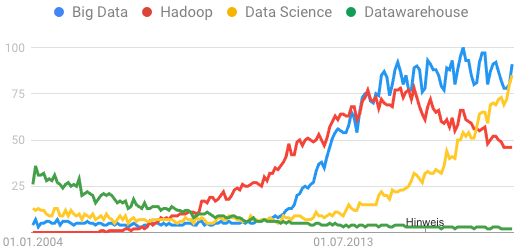
\includegraphics[width=1.0\textwidth]{google_trends_bigdata.png}
	\caption{Schema - Google Trends (Popularity Of Certain Search Terms)}
	\label{google_trends_bigdata}
\end{figure}


\section{Distributed Computing}
\label{bd_hwe}

CPU RAM Vertical to horizontal Scalability --> Distributed Computing
Data volume increases
Data processing increases
Scale out vs Up
Cloud provider 
- Lets rent a super computer
Cloud vs Custer Computing
Containerization
MapR IaaS, PaaS, SaaS


to-be-added

\newpage
\section{BigData V's}
\label{bd_vs}
Firstly introduced by Gartner in 2011\footnote{\cite{GRTNRVS}, https://www.gartner.com/newsroom/id/1731916} the (initial) \textit{3 V's of Big Data} quickly became key characteristics and challenges of Big Data. Back in this time the focus on Big Data was on the volume of data alone, ignoring the \textit{variety} of information (databases, documents, video, social media) and \textit{velocity} of information (how fast it is being produced and how fast it needs to be processed) as well. \\
Today some more V's have established (Figure \ref{bigdata_vs}), we will quickly disscuss them within the next chapters.

\begin{figure}[ht]
	\centering
  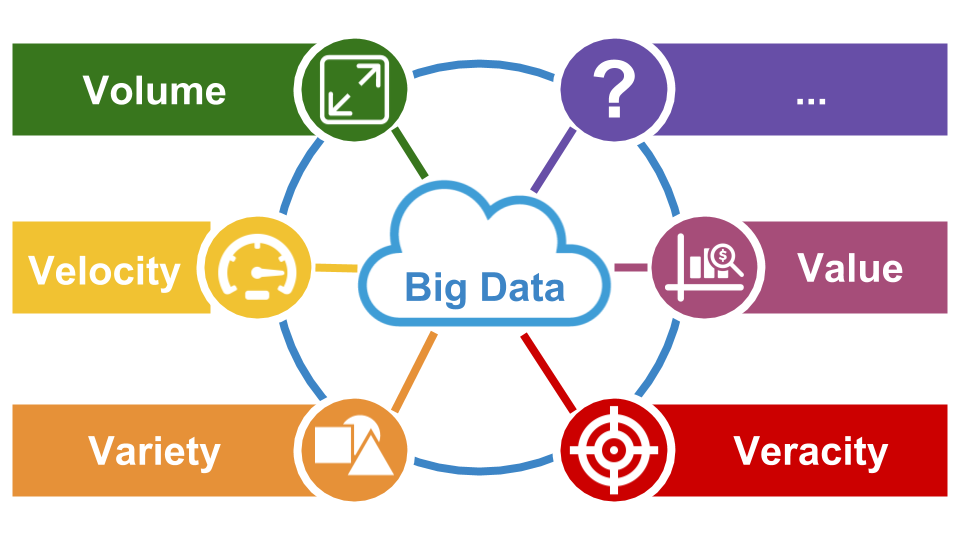
\includegraphics[width=0.8\textwidth]{bigdata_vs.png}
	\caption{Schema - Big Data V's}
	\label{bigdata_vs}
\end{figure}

\subsection{Volume}
\label{bd_vs_volume}
\textit{Volume} sounds quiet obvious as we are talking about Big Data, but what is Big in terms of volume? Let's have a quick look at some examples: 
\begin{itemize}
	\item \textbf{Wikipedia:} in 2014 the english part of Wikipedia as well as Wikipedia Commons (including Media like Images, Videos etc.) had a size of around 23TB\footnote{\cite{WPS}, https://en.wikipedia.org/wiki/Wikipedia:Size\_of\_Wikipedia}.
	\item \textbf{Spotify:} in 2013 data generated by users of was about 1,5TB per day which approximately means 534TB per year\footnote{\cite{SPTFYV}, https://de.slideshare.net/AdamKawa/big-data-at-spotify}.
	\item \textbf{Google:} the search index currently has a size of 100PB\footnote{\cite{GSIS}, https://www.google.com/search/howsearchworks/crawling-indexing/}.\\
\end{itemize}

But Big Data does not need to be about those kind of sizes. As a rule of thumb, data that can easily be handled (e.g. processed, saved or queried) within a traditional database (e.g. PostgreSQL, Informix, DB2, Oracle etc.) and belonging datawarehouse, like a few gigabytes per week or month, is not Big Data. \\
But it's not unlikely that there is an adequate Big Data case in your immediate surrounding, for instance if you are running a mid-level e-commerce shop and make use of tracking data like web server log files (e.g. produced by Apache, Nginx) or data provided by third-party tracking tools like Google Analytics or WebTrekk with the aim to analyze the behaviour of visitors of your website, you easily end up with several terabytes of logfiles/tracking data per year, which needs to be processed. If you would like to calculate cohorts or a CLV\abk{CLV}{Customer Lifetime Value}\footnote{\textit{CLV - Customer Lifetime Value, prediction model which calculates the net profit attributed to the entire future relationship with a customer based on the past}} this would even require processing the data of several years and in this way probably more than 10TB of data at once.


\subsection{Velocity}
\label{bd_vs_velocity}
\textit{Velocity} in terms of Big Data has two facets: how fast data is produced and how fast it needs to be processed to be able to make use of or react to it. Depending on the use case it is required to react within minutes or even seconds. Let's have a quick look at some examples: 

\begin{itemize}
	\item \textbf{Facebook:} in 2012 every 60 seconds 510.000 comments, 293.000 status updates and 136.000 photos had been posted on average, which needed to be processed in near real-time\footnote{\cite{TSSFP}, http://thesocialskinny.com/100-social-media-statistics-for-2012/}.
	\item \textbf{Twitter:} in 2013 usually 500 million tweets were posted each day on Twitter, which means 5.7000 Tweets per second on average\footnote{\cite{TWTTPS}, https://blog.twitter.com/engineering/en\_us/a/2013/new-tweets-per-second-record-and-how.html}.
	\item \textbf{Google:} According to Internet Live Stats, Google is handling around 6 billion search requests per day, which approximately means 70.000 per second.\footnote{\cite{ILSGS}, http://www.internetlivestats.com/google-search-statistics/}.\\
\end{itemize}

But your data-system does not need to handle those kind of velocities to be called BigData. For instance if your working for mid-level bank like ING Netherlands, you need to handle 1 million transactions per day, which is ``just'' 12 requests per second. But those requests need to be handled in real-time. Additionally during the processing of those requests (transactions) several data science models need to be involved and executed to be able to detect fraudulent transactions as they happen, to protect the bank and its customers. ING Netherland achieves this by using Apache Kafka\footnote{\cite{KAFKAHP}, https://kafka.apache.org/} for queuing events and streaming them into Apache Flink\footnote{\cite{FLINKHP}, https://flink.apache.org/} to apply machine learning models\footnote{\cite{DAING}, https://data-artisans.com/blog/real-time-fraud-detection-ing-bank-apache-flink}. \\
Real-time data processing and running data science models on it, is not just a case for the big players like Facebook, Twitter and Google, for instance fraud detection on transactions is also quiet interesting if your company runs a mid-level e-commerce shop or if it is an insurance company as well. If you run a website and want to customize the content in real-time, so that a visitor sees what he would like to see (based on his previous behaviour on the website) you probably end up with \textit{onsite-personalization} which also requires real-time data processing and applying data-science models. \\
This is just a glimpse of characteristics, challanges and possible use cases in terms of data \textit{velocity} and Big Data.

\subsection{Variety}
\label{bd_vs_variety}
\textit{Variety} refers to the diversity of data sources, so called ``Big Data'' data-systems need to handle. Those data sources and their structures are widely diversified and cannot easily be handled by traditional relational databases. Let's have a look at a few examples and put them into 3 well known categories: \textit{structured data}, \textit{semi-structured data} and \textit{utructured data}.\\


\begin{itemize}
	\item \textbf{Structured Data:} means plain data structures which have fixed attributes/columns, specific data types and a defined domain. Related but different kinds of data records can easily be linked using constraints of the relational data model, like primary and foreign keys. This kind of data can easily (almost directly) be stored into a traditional SQL database or similar.\\
	\item \textbf{Semi-Structured Data:} covers all data structures, that do not easily fit into the constraints of the relational data model and in this way into a relational SQL database. Even though semi-structured data has of course some organizational properties that makes it easy to categorize, link and analyze the data. With ``some'' additional work it is possible to store this kind of data in a relational SQL database, but as this will violate many constraints of the relational data model, you would end up making a lot of compromises, e.g. in terms of defined domains, expected structures, or extensibility which do not fit very well into the relational world or only with a lot of operational overhead and workarounds. Semi-structured data has some structure in terms of tags and attributes but those and nested structures as well will usually change from document to document or data record to record. The semi-structured data model has some serious advantages: no need to worry about \textit{object-relational impedance mismatch} and support for highly nested and hierarchical data and in this way simplified data models but it is also more prone to \textit{``grabage-in, garbage-out''} as important constraints of the relational model are thrown away. Examples of semi-structured data are:
	\begin{itemize}
		\item \textbf{JSON} documents (e.g. provided by the Facebook Graph API\footnote{\cite{FBGAPI}, https://developers.facebook.com/docs/graph-api/using-graph-api/} or the Twitter API\footnote{\cite{TWTAPI}, https://developer.twitter.com/en/docs/tweets/data-dictionary/overview/tweet-object.html}), 
		\item \textbf{XML} documents (e.g. provided by the Google Maps Geocoding API\footnote{\cite{GMGCAPI}, https://developers.google.com/maps/documentation/geocoding/intro} or the OpenWeatherMap Weather API\footnote{\cite{OWMAPI}, https://openweathermap.org/api}) or
		\item \textbf{HTML} documents, for instance if your developing a web crawler (e.g. using Scrapy\footnote{\cite{SCPYHP}, https://scrapy.org/} for data gathering or Selenium\footnote{\cite{SELEHP}, https://www.seleniumhq.org/} for testing purposes).\\
	\end{itemize}
	\item \textbf{Unstructured Data:} is everything that is neither structured or semi-structured. This usually includes:
	\begin{itemize}
		\item \textbf{Natural language}, for instance Social Media Posts (e.g. Facebook and Twitter), Ratings (e.g. on Amazon, IMDB or other platforms) or plain text (e.g. Wikipedia articles, product information on Amazon or any e-commerce shop) you may want to analyze by \textit{natural language processing} with the purpose of calculating a sentiment (\textit{What do customers think about your product?}) or the meaning and truthfulness of a rating (\textit{Is the review positive or negative? Is it fake?}). 
		\item \textbf{Geographical data}, for instance satellite, GPS, radar or sonar data and images with the purpose of analyzing meteorological, vecicular or seismic behaviour, e.g. for the purpose of predicting the future.
		\item \textbf{Photos and Videos}, for instance of traffic and surveillance cameras to analyze and optimize traffic flow or for the sake of security.
		\item \textbf{Scientific data}, like physic measuring and sensor data, seismic imagery or athmospheric data to analyze and optimize a physics experiment. For instance CERN makes use of Hadoop for unstructured sensor data, to unlock insights from machine data\footnote{\cite{CERNH}, https://conferences.oreilly.com/strata/stratany2014/public/schedule/detail/36312}
		\end{itemize}
\end{itemize}

\subsection{Veracity}
\label{bd_vs_veracity}
Speaking about Big Data, \textit{veracity} is about the trustworthiness and accuracy of a certain dataset. Especially in terms of accuracy it is not just about the quality of the data itself, but also tasks of quality assurance and data cleansing, like removing bias, superfluous, redundant or just duplicate records or attributes. Trustworthiness is also highly vulnerable to the volatility of the data (which you usually cannot control), as a lot of data sources and related records frequently change in their lifetime. For instance an account balance quickly changes over time (due to ongoing transactions) as well as people which have liked a topic, post or site on a social media platform may dislike it the next day. Additionaly there are a lot more possible mistakes, caused by humans or machines, like wrong system timestamps, an incomplete or corrupted dataset may causing a complete different result. Even if you have a fully-fletched environment which ensures data quality in its own limits, you cannot be sure the data you are processing is 100\% accurate, as their could already be a mistake in the source system. For instance if you are processing data from a tracking system and you are able to ensure 100\% completeness of data and accuracy within your ETL processes (e.g. using automated tests like FitNesse\footnote{\cite{FITNHP}, http://docs.fitnesse.org/FrontPage}), their could already be a significant bias in the source system, as a related tracking pixel may not have been properly configured on every page of your e-commerce shop (e.g. due to a relaunch of your website), so you are maybe missing some page views and products viewed in your tracking data. Or much simpler, an issue that even the tracking sytsem cannot handle: people who disable third party cookies, they will always appear as new visitors in your tracking data, even if its the 10th time they visit your e-commerce shop. \\
As analytics and related conclusions rely on the quality of the data, a Big Data data-system should always try to achieve the best data quality possible, even it is seen a lot: \textit{Garbage In - Garbage Out} is not acceptable.


\subsection{Value}
\label{bd_vs_value}
Last but probably most important of all V's is the \textit{value}. We previously discussed \textit{volume}, \textit{velocity}, \textit{variety} and \textit{veracity} - all of them are meaningless if you dont derive business \textit{value} from your data, but they are also significant enabler and success factors for the \textit{value} of your data. We will quickly discuss the correlation now: 
\begin{itemize}
	\item \textbf{Volume:} the more data you collect, the more insights you can probably gather and the more informed your insights and decisions may be. But its not only about the volume, if your company does not have the ressources and capabilities to perform the required analysises on collected data and perform the derived actions, \textit{volume} is menaingless.
	\item \textbf{Velocity:} Today everything is about speed, especially business. The faster data is collected and available for analysis processes, the faster it can be used for decision-making processes.
	\item \textbf{Variety:} The more data sources you connect to your data-system, the more insights you can potentially create and probably you will no longer rely an a single data source for a certain business object (like a client), which overall increases data quality and depth. Enabling you, for instance to build customer journeys, calculate a CLV, and in this way improve engagement and retention. At the end the \textit{value} of your data increases.
	\item \textbf{Veracity:} This is quiet obvious, as the more trustworthy and accurate your data is, more business critical desicisions and applications will rely on it and in this way the revenue of your company will probably increase as well as the value of your data.\\ 
\end{itemize}

\textit{Value} can probably be found in any kind of data, but the challenge is to pick the right data and use it the right way. First of all you need to understand the potential, benefits and have an idea of what you want to achieve. For instance use it to understand your customers better, (re-)target them accordingly in advertisements or increase engagement by onsite-personalization and recommendation engines. Maybe you want to optimize processes or machine and ressource utilization or just analyze log files to identify security violations or netwerk performance issues. There is an infinite number of cases a Big Data data-system can create business value. \\
If you just do not want to throw data away, there are cheaper and more appropriate solutions than a Big Data data-system. 

\subsection{Other V's}
\label{bd_vs_other_vs}
to-be-added

\section{Big Data Challenges}
\label{bd_def}
to-be-added

\section{Big Data And Consistency}
\label{bd_consistency}

\subsection{CAP Theorem}
\label{bd_consistency_cap}

\subsection{ACID Theorem}
\label{bd_consistency_acid}

\subsection{BASE Theorem}
\label{bd_consistency_base}

\section{Big Data in Business}
\label{bd_bdib}
to-be-added

\subsection{Big Data Use Cases}
\label{bd_bdib_ucases}
to-be-added

\subsection{Big Data Analytics Value Chain}
\label{bd_bdib_vchain}

\subsection{Roles}
\label{bd_bdib_roles}
Within this chapter we will get a quick overview of the most common job roles required to build a Big Data data-system as well as a general understanding of their required skillsets, tasks and responsibilities.

\subsubsection{Data Engineer/Architect}
\label{bd_bdib_roles_de}
\textit{Data Engineers/Architects} are designer, builder and manager of the information of a Big Data data-system. A Data Engineer develops, tests, maintains and improves highly scalable data-systems. Development includes ETL Jobs, custom analytics applications or custom software components for standard analytic tools. A data engineers work is all about collecting, transforming and storing data, this can be achieved using batch processing or real-time streaming, with the goal to serve analytical use cases, applications and data scientists.
\\Sometimes a Big Data Architect is a separate Job role but most of the time, especially in smaller companies, it is part of a Data Engineers work. Usually someone more senior, for instance a Lead Data Engineer takes responsibility of architectural tasks and responsibilities, ensures long-term quality and flexibility of the software the team develops, shares best practices with team and enables the team to meet their goals and be successful.\\
\begin{itemize}
	\item \textbf{Study Direction:} Computer Science (databases, software engineering, distributed systems and processing, real-time processing)\\
	\item \textbf{(Programming) Languages:} Java, Scala, Python, Bash, if necessary ETL Tools (e.g. Pentaho Data Integration, Informatica, DataStage, Talend)\\
	\item \textbf{Key Skills:} 
		\begin{itemize}
		\item data modeling
		\item ETL and dataflow architecture and design
		\item data pipelin/workflow design and management
		\item stream- and batch-processing
		\item understand the concept, performance factors and limitations of distributed data-systems
		\item alignment with larger organizations goals and strategy as well as corporate guidelines (e.g. data protection, information security, license and toolset policies)\\
		\end{itemize}
	\item \textbf{Tasks:} 
		\begin{itemize}
		\item develop ETL jobs, data- and workflows
		\item develop and define architecture of a data-system, 
		\item integration of data-sources
		\item alignment with larger organizations goals and strategy as well as corporate guidelines (e.g. data protection, information security, license and toolset policies)\\
		\end{itemize}
\end{itemize}

\subsubsection{Data Ops}
\label{bd_bdib_roles_ops}
A \textit{Data Operations Manager} (also known as Ops Manager) is an integral part of the whole big data team. An Ops manager will ensure that productive data-systems and services continually meet business needs in a reliable and efficient manner. This role requires strong communications as well as technical skills around incident and problem management, but mainly infrastructure and software deployment, configuration, automation and monitoring. An Ops manager will assess and analyze complex infrastructure and data problems and provide solutions that meet the companies objectives while working closely together with Data Engineers and Data Scientists.\\

\begin{itemize}
	\item \textbf{Study Direction:} Computer Science (databases, software engineering, distributed systems and processing, real-time processing)\\
	\item \textbf{(Programming) Languages:} Python, Bash\\
	\item \textbf{Key Skills:} 
	\begin{itemize}
	\item strong communication and collaboration skills
	\item broad knowledge of Ops Tools, best practices and automation
	\item frequently refreshs his knowledge as Ops tools crop up continuosly 
	\item Continuos Integration and Deployment Automation (e.g. Jenkins, Gitlab CI), 
	\item Infrastructure Automation (e.g. Foreman, Puppet, Ansible), 
	\item Containerization (e.g. Docker, LXD etc.), 
	\item Orchestration (e.g. Kubernetes, Mesos, Swarm),
	\item Cloud (e.g. AWS, Google Cloud Platform, Azure, OpenStack)
	\item Source Control (e.g. Git, Bitbucket, SVN)\\
	\end{itemize} 
	\item \textbf{Tasks:} 
	\begin{itemize}
	\item installs, configures, upgrades, scales and operates infrastructure and applications
	\item monitoring and management of infrastructure and applications
	\item provides and manages tools for continues delivery
	\item incident and problem management
	\item interface to developers (requirements for infrastructure, support developers needs and productive application operation)\\
	\end{itemize} 
\end{itemize}

\subsubsection{Data Scientist}
\label{bd_bdib_roles_ds}
A \textit{Data Scientist} is responsible for interpreting data, extracting and discovering insights from strcutured and unstrcutured data to meet specific business needs and goals. Therefore a data scientist will analyze (probably a large) amount of data, make use of statistics, machine learning as well as belonging software and libraries specifically designed for his job. A data scientists needs to have enough business domain expertise and deep understanding of the data he is working with as well as strong communication and presentation skills to be able to easily share his insights with his stakeholders (usually business outside of IT).\\

\begin{itemize}
	\item \textbf{Study Direction:} Statistics, Data Science, Mathematics, Computer Science (Java, Python, R, SQL, Machine Learning) \\
	\item \textbf{(Programming) Languages:} Python, R, Matlab, Bash, Java, Scala\\
	\item \textbf{Key Skills:} 
	\begin{itemize}
	\item strong communication and collaboration skills
	\item business domain expertise
	\item deep understanding of the data he is working with
	\item broad experience in using programming languages and tools for statistical purposes (Python, R, SQL, MapReduce, Spark, SparkML, Pandas, dataframes)
	\item knowledge of a variety of machine learning techniques (e.g. clustering, regression, decision trees, neural networks, properties of distribution)
	\item strong skills in data visualization (e.g. seaborn, Matplotlib, ggplot)\\
	\end{itemize} 
	\item \textbf{Tasks:} 
	\begin{itemize}
	\item identify and evaluate data-analytics problems that offer the greatest opportunities and/or business value
	\item determining the right data sets and variables
	\item cleansing and validation of data to ensure completeness, accuracy and uniformity
	\item developing and applying models and algorithms on data 
	\item analyze data to identify patterns, risks and trends
	\item commmunication with and visualization for (business) stakeholder\\
	\end{itemize} 
\end{itemize}


Obviously there are far more job roles required to build and operate a data-system, for instance Product Owner, Scrum Master, Business or Data Analysts. But as their required skillset is not very specific to Big Data, unlike the previously discussed job roles, we won't go into detail here.

\subsection{BI vs DataScience}
\label{bd_bdib_bi_vs_datascience}
to-be-added


\subsection{Dissociation Datawarehousing}
\label{bd_bdib_diss_dwh}
to-be-added

\section{Definition of Big Data}
\label{bd_def}
to-be-added
\\[0.5 cm]
\hspace*{4mm}%
\fbox{%
  \hspace*{1.5mm}\hspace*{-1\fboxsep}%
  \parbox{0.08\textwidth + 5mm - 2\fboxsep}{%
\begin{minipage}{0.1\textwidth}
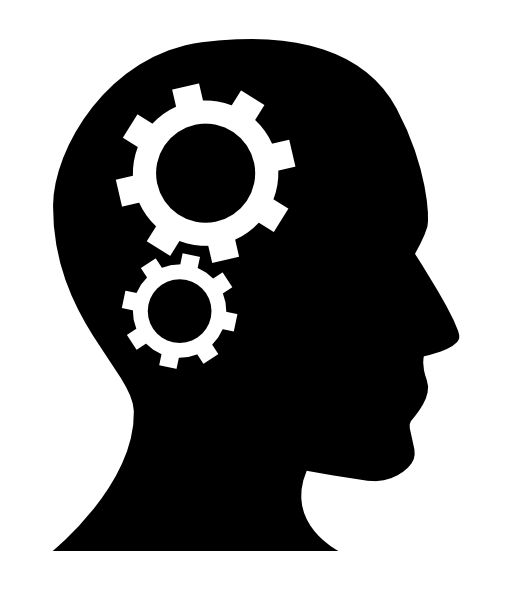
\includegraphics[width=\linewidth]{gear_brain.png}
\end{minipage}
  }%
}\hspace*{4mm}%
\begin{minipage}{0.8\textwidth}\raggedright
\textbf{BigData} is a term for data sets that are so large or complex that traditional database management tools or data processing software is inadequate to deal with them. \\
\end{minipage}\\[0.4 cm]

\section{Big Data Science}
\label{bd_science}
to-be-added